\documentclass[11pt,UTF8]{ctexart}
\title{圆形固体在库埃特与泊肃叶流下的数值模拟情况}
\author{马坤}
\date{2020.1.28}
\usepackage{amsmath}
\usepackage{graphicx}
\usepackage{caption}
\usepackage{subcaption}
\usepackage[left=1in, right=1in, top=1in, bottom=1in]{geometry}
\begin{document}
    \maketitle
    \par{在流体中的圆形固体指的是在正方形流体区域有一个
    圆心在中心的固体,我们在此模拟中将其看成一个可以粘性
    较大的流体。假设正方形区域高为$H=1$,长为$L=1$。
    圆形位于$(1/2,1/2)$,半径长$R=1/4$。进一步假设刻画流体
    区域的示性函数,
    $$\phi=\tanh \frac{2.4(r-1/4)}{W},r=\sqrt{(x-1/2)^2+(y-1/2)^2}$$
    $\phi$理应($W$较小)粘性较大流体(圆形区域内$r<R$)里面为1,理应($W$较小)在粘性
    较小流体(圆形区域外$r>R$)里面为0。}
    \par{模拟中我们假设粘性比$\frac{\eta_s}{\eta_l}=rate$,其中
    $\eta_s$为较大的粘性(圆形的区域内的流体),$\eta_l$为较小的
    粘性(圆形的区域外的流体),无维度化后的粘性系数$\eta$有如下表达式:
    $$\eta = 1+rate*\phi-\phi.\eqno(2)$$
    上述两个表达式上面两个表达式中的$W,rate$都是待定的参数,接下来
    会通过实验选取较好的值。实验中假设的流体的密度均为$\rho=1$,所以
    有$\eta=\nu$。}
    \section{库埃特流}
    \par{面对库埃特流目前就只实验了一个情况,$W=0.1,rate=50$。下图为3维
    的情况与2维的情况。其中2维图中$x=0,x=0.5$意味着截取的平面为长的开始点
    $(0,0)$与中间点$(L/2,0)$。}
    \begin{figure}[h]
        \centerline{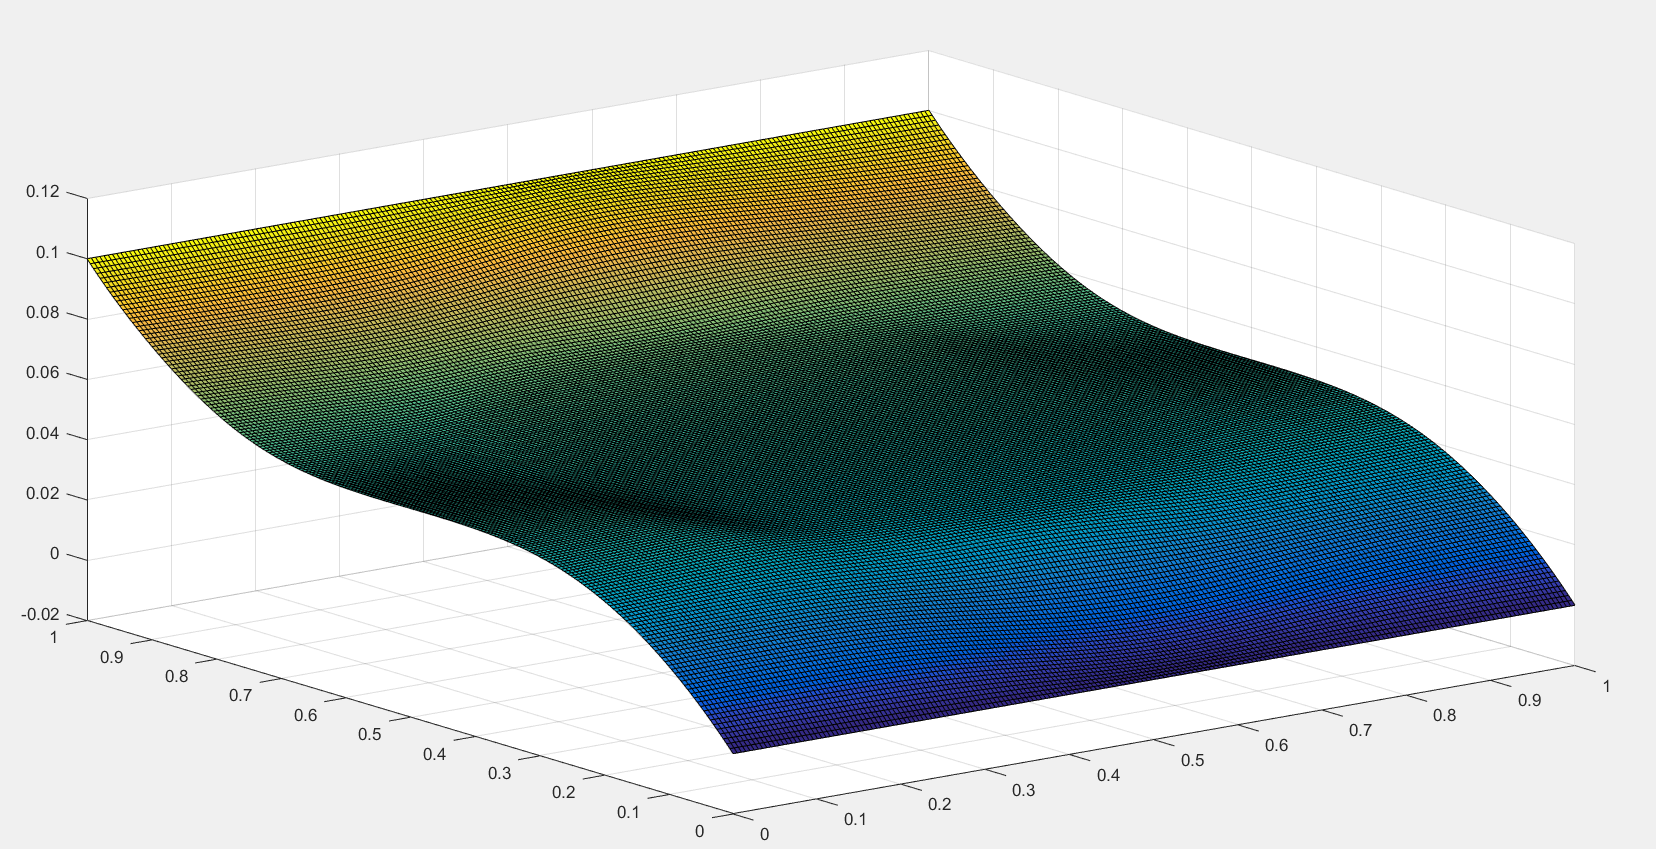
\includegraphics[width=0.8\textwidth]{cutte_W_3D.png}}
        \caption{库埃特流的3D图像}
    \end{figure}
    \begin{figure}[h]
        \centerline{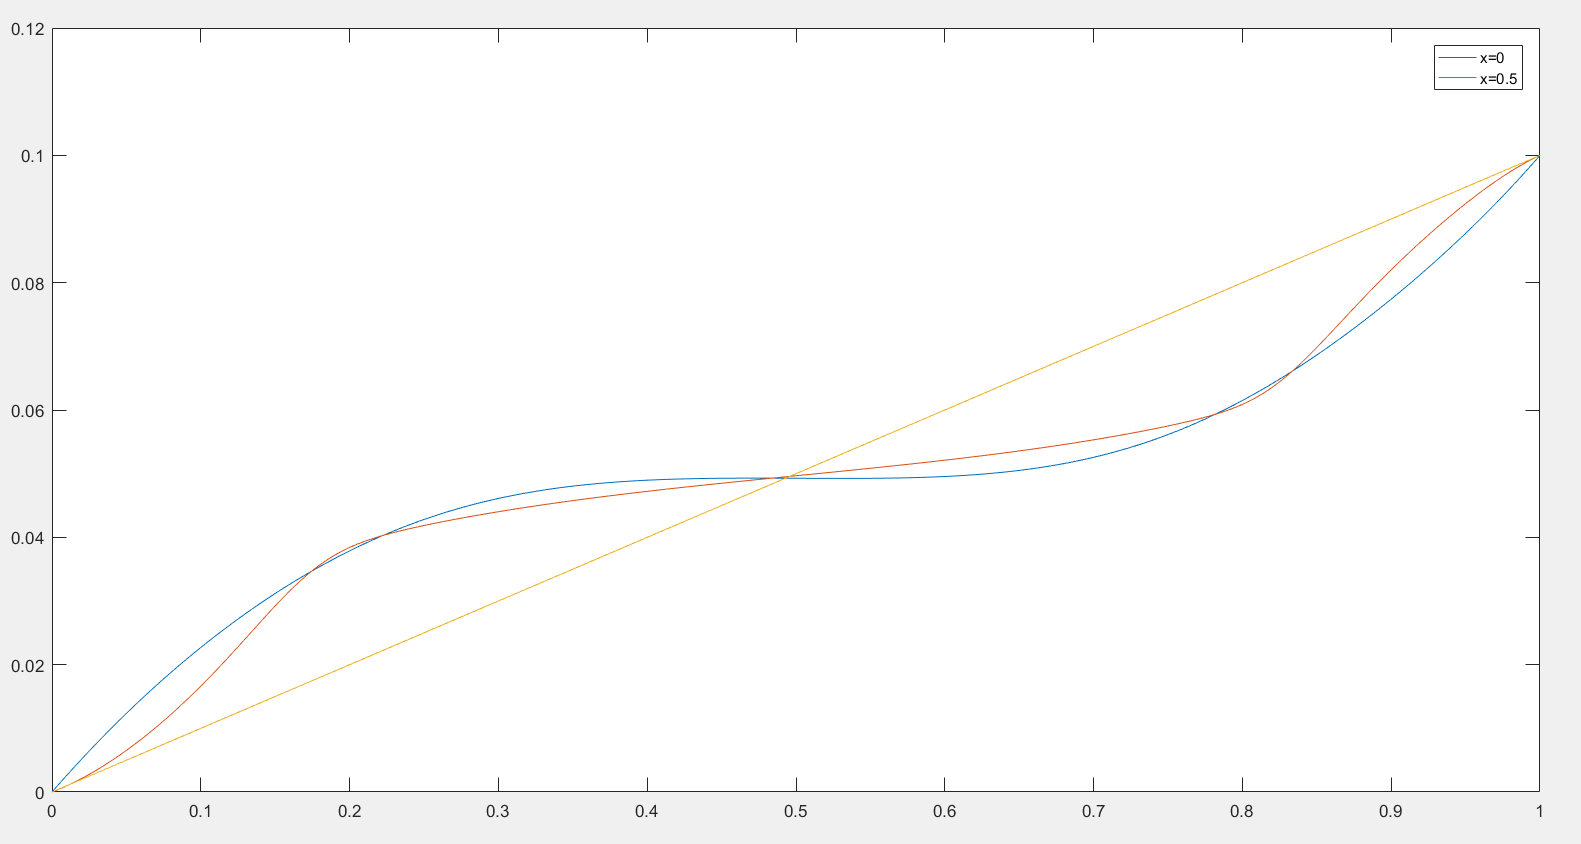
\includegraphics[width=0.8\textwidth]{cutte_W_2D.png}}
        \caption{库埃特流的2D图像}
    \end{figure}
    \section{泊肃叶流}
    \par{面对库埃特流目前就只实验了一个情况,$W=0.1,rate=50$。正如
    之前,此时力是恒定的,所以其选取就有了一定麻烦。当力取得较大$F=\frac{8\rho u_{peak} \eta_s}{H^2}$时,
    数值算法崩溃了,当取得较小时$F=\frac{8\rho u_{peak} \eta_l}{H^2}$,
    稳定结果如下。其中2维图中$x=0,x=0.5$意味着截取的平面为长的开始点
    $(0,0)$与中间点$(L/2,0)$。}
    \begin{figure}[h]
        \centerline{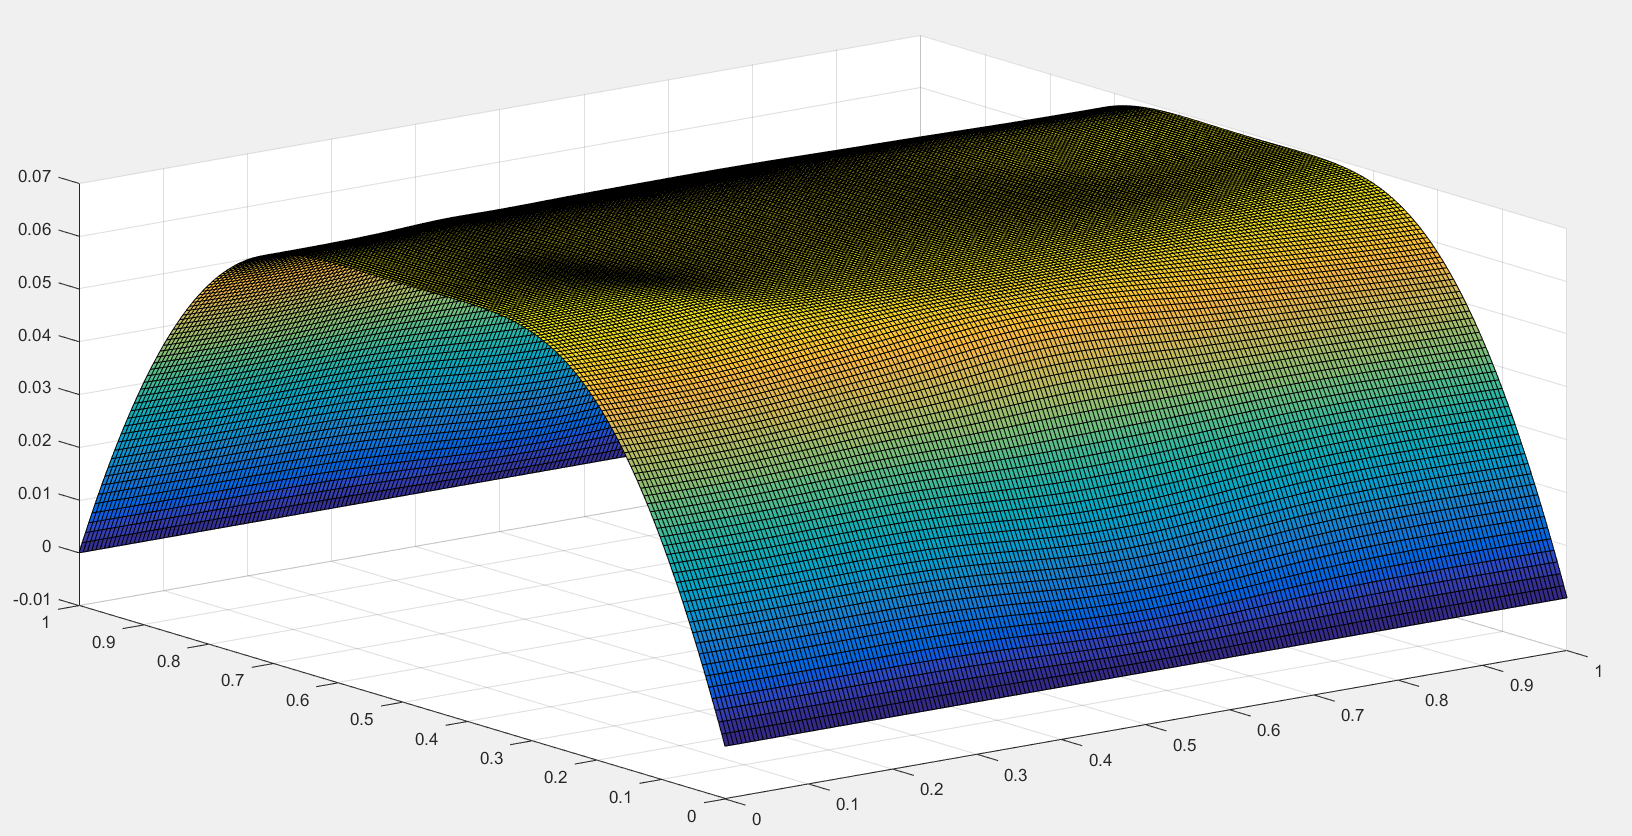
\includegraphics[width=0.8\textwidth]{P_3D.png}}
        \caption{泊肃叶流的2D图像}
    \end{figure}
    \begin{figure}[h]
        \centerline{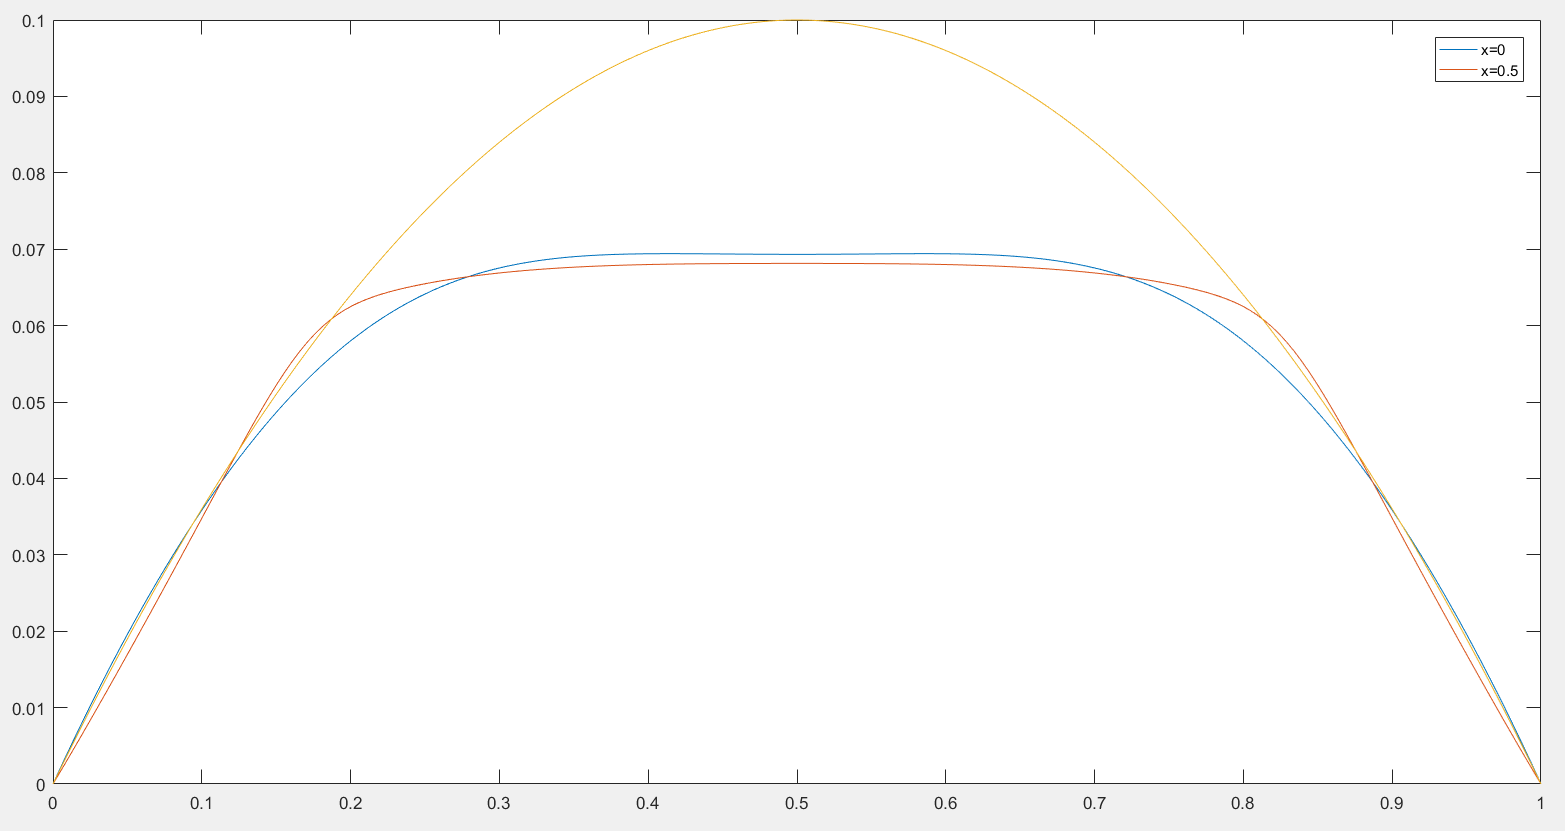
\includegraphics[width=0.8\textwidth]{P_2D.png}}
        \caption{泊肃叶流的2D图像}
    \end{figure}
\end{document}